% !TeX root = Report.tex
\section{Results}

\subsection{Methodology}

In our simulations we tested networks of various sizes (15, 30 and 48 nodes) aligned in a grid. The nodes were placed such that every node had four neighbours, one to the north, south, east and west, except for nodes in the edge which had three neighbours and the nodes in the corner that had two neighbours. The sink was always placed in the top left corner and was always assigned the address ``1.0''. The predicate checking algorithm was started as soon as the nodes had come online, the nodes then waited for 5 minutes to allow the predicate checking algorithm time to setup and then the TDMA algorithm was started. The simulation was run for 35 minutes overall and then it was terminated. After the predicate checking algorithm had setup the predicate was checked every 4 minutes.

To gather metrics on the energy usage of the motes, a Contiki library called rimestats was used. This library is built into the MAC layer and records deep statistics, we simply used the sent and received message counts. In order to calculate how much energy the TDMA algorithm was using we implemented our own sent and received counters that were incremented when a message was sent or received. As the TDMA protocol was implemented with simple broadcasts there should be a one-to-one correspondence between the number of successful broadcasts and the number of transmissions done at the MAC layer, the same is also true for when receiving a message. To calculate the energy cost of the predicate evaluation algorithm, the different between the total and the TDMA energy usage was taken.

To check that a predicate was successfully evaluated the TDMA algorithm printed any changes in the assigned slot as well as the time the slot was changed. When a predicate was evaluated on a node the time it was evaluated as well as the result was printed. Analysis scripts then evaluated the predicate using the most recent slot value from before or up to when the predicate was evaluated to evaluate the predicate itself. This result was then compared with the actual result of the predicate. The results were compared whether or not the predicate response message reached the sink.


\subsection{Graphs}

\begin{figure}[ht]
\centering
\subfigure[Rx]{%
	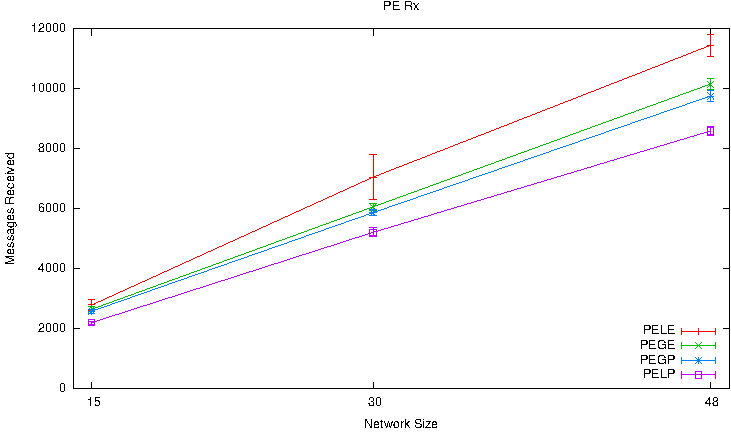
\includegraphics[width=0.44\linewidth]{../Results/Graphs/4.0/1HOP/messagesPE/rx/graph.pdf}
}
\subfigure[Tx]{%
	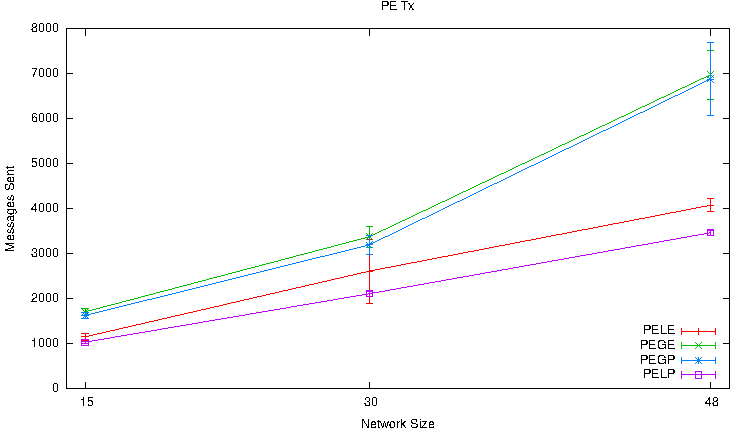
\includegraphics[width=0.44\linewidth]{../Results/Graphs/4.0/1HOP/messagesPE/tx/graph.pdf}
}

\subfigure[Percentage of  predicates correctly evaluated]{%
	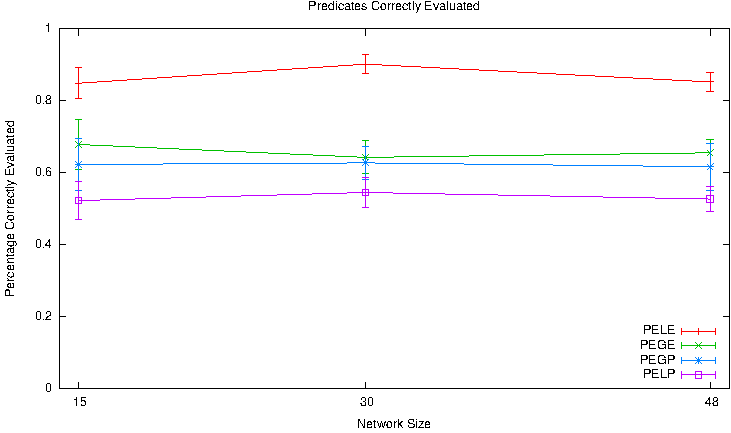
\includegraphics[width=0.44\linewidth]{../Results/Graphs/4.0/1HOP/pcCorrectlyEvaluated/graph.pdf}
}
\subfigure[Percentage of responses received]{%
	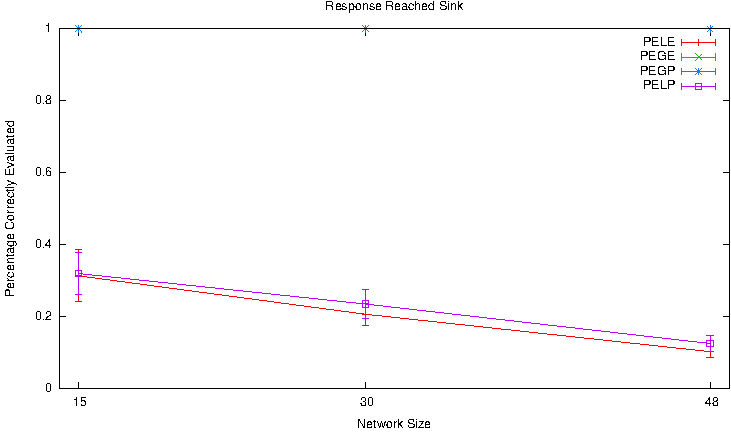
\includegraphics[width=0.44\linewidth]{../Results/Graphs/4.0/1HOP/pcResponsesReachedSink/graph.pdf}
}
\caption{Results when predicate period is every 4.0 seconds}
\end{figure}

\begin{figure}[ht]
\centering
\subfigure[Rx]{%
	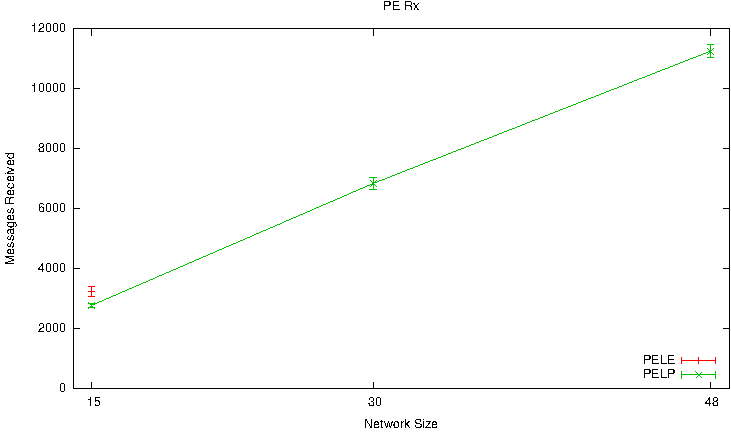
\includegraphics[width=0.44\linewidth]{../Results/Graphs/2.0/1HOP/messagesPE/rx/graph.pdf}
}
\subfigure[Tx]{%
	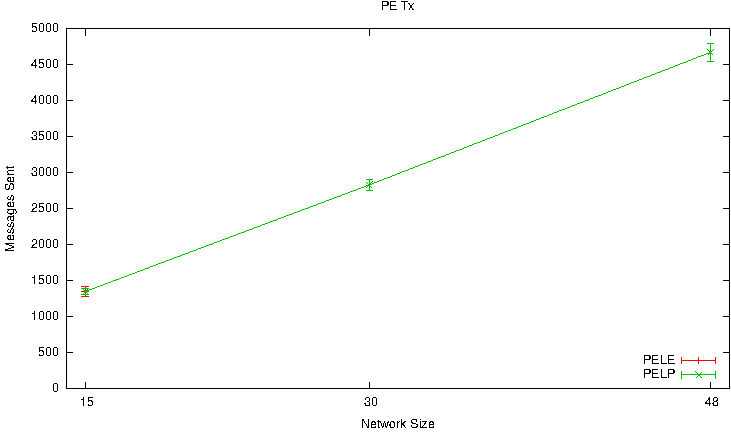
\includegraphics[width=0.44\linewidth]{../Results/Graphs/2.0/1HOP/messagesPE/tx/graph.pdf}
}

\subfigure[Percentage of predicates correctly evaluated]{%
	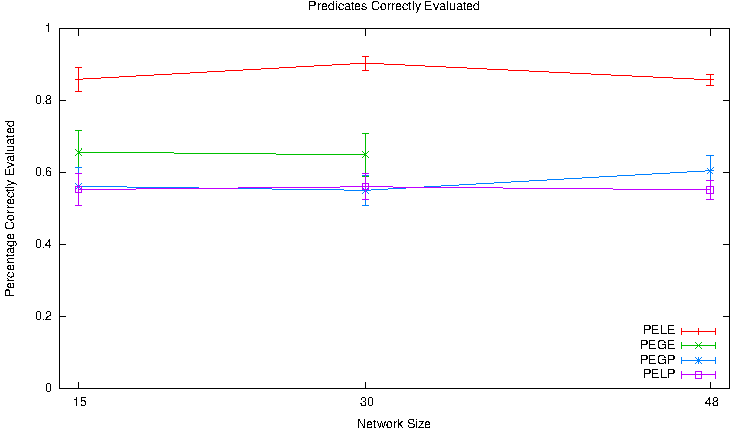
\includegraphics[width=0.44\linewidth]{../Results/Graphs/2.0/1HOP/pcCorrectlyEvaluated/graph.pdf}
}
\subfigure[Percentage of responses received]{%
	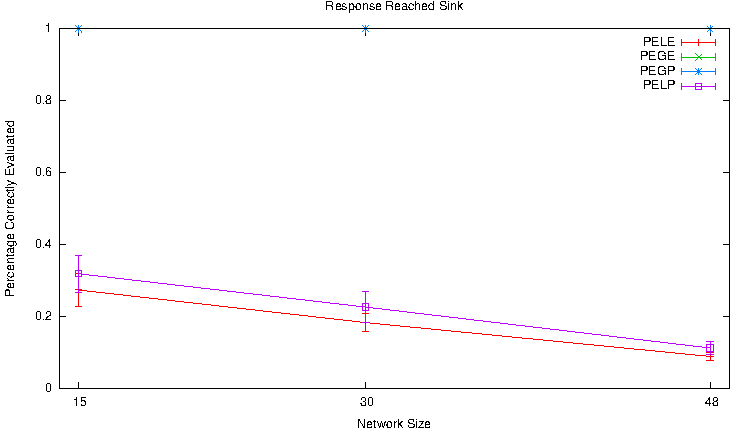
\includegraphics[width=0.44\linewidth]{../Results/Graphs/2.0/1HOP/pcResponsesReachedSink/graph.pdf}
}
\caption{Results when predicate period is every 2.0 seconds}
\end{figure}

